\documentclass[twoside,accentcolor=tud2a,nochapname,11pt]{tudexercise}
\usepackage{listings}
\usepackage{hyperref}
\usepackage{upgreek}

\title{A handheld hall probe based on an Arduino Micro}
\subtitle{Application for \textit{Arduino Uno WiFi XMAS Contest 2015}}
\subsubtitle{by Henning Janssen}

\begin{document}

\maketitle

This is a short documentation about a mobile handheld hall probe, which is based on an Arduino Micro.
A battery powered Arduino evaluates via the analog input a hall effect sensor. The measured value will be shown on a display.

With this device it is possible to measure magnetic fields, i.e. the magnetic flux density as a constant and as a time-depending value. It is portable and independent from a power grid.

\section{Hardware}

The total system consists of a handheld (includes the Arduino, energy supply and display) and a set of external sensors.
\begin{figure}[ht]%
\centering
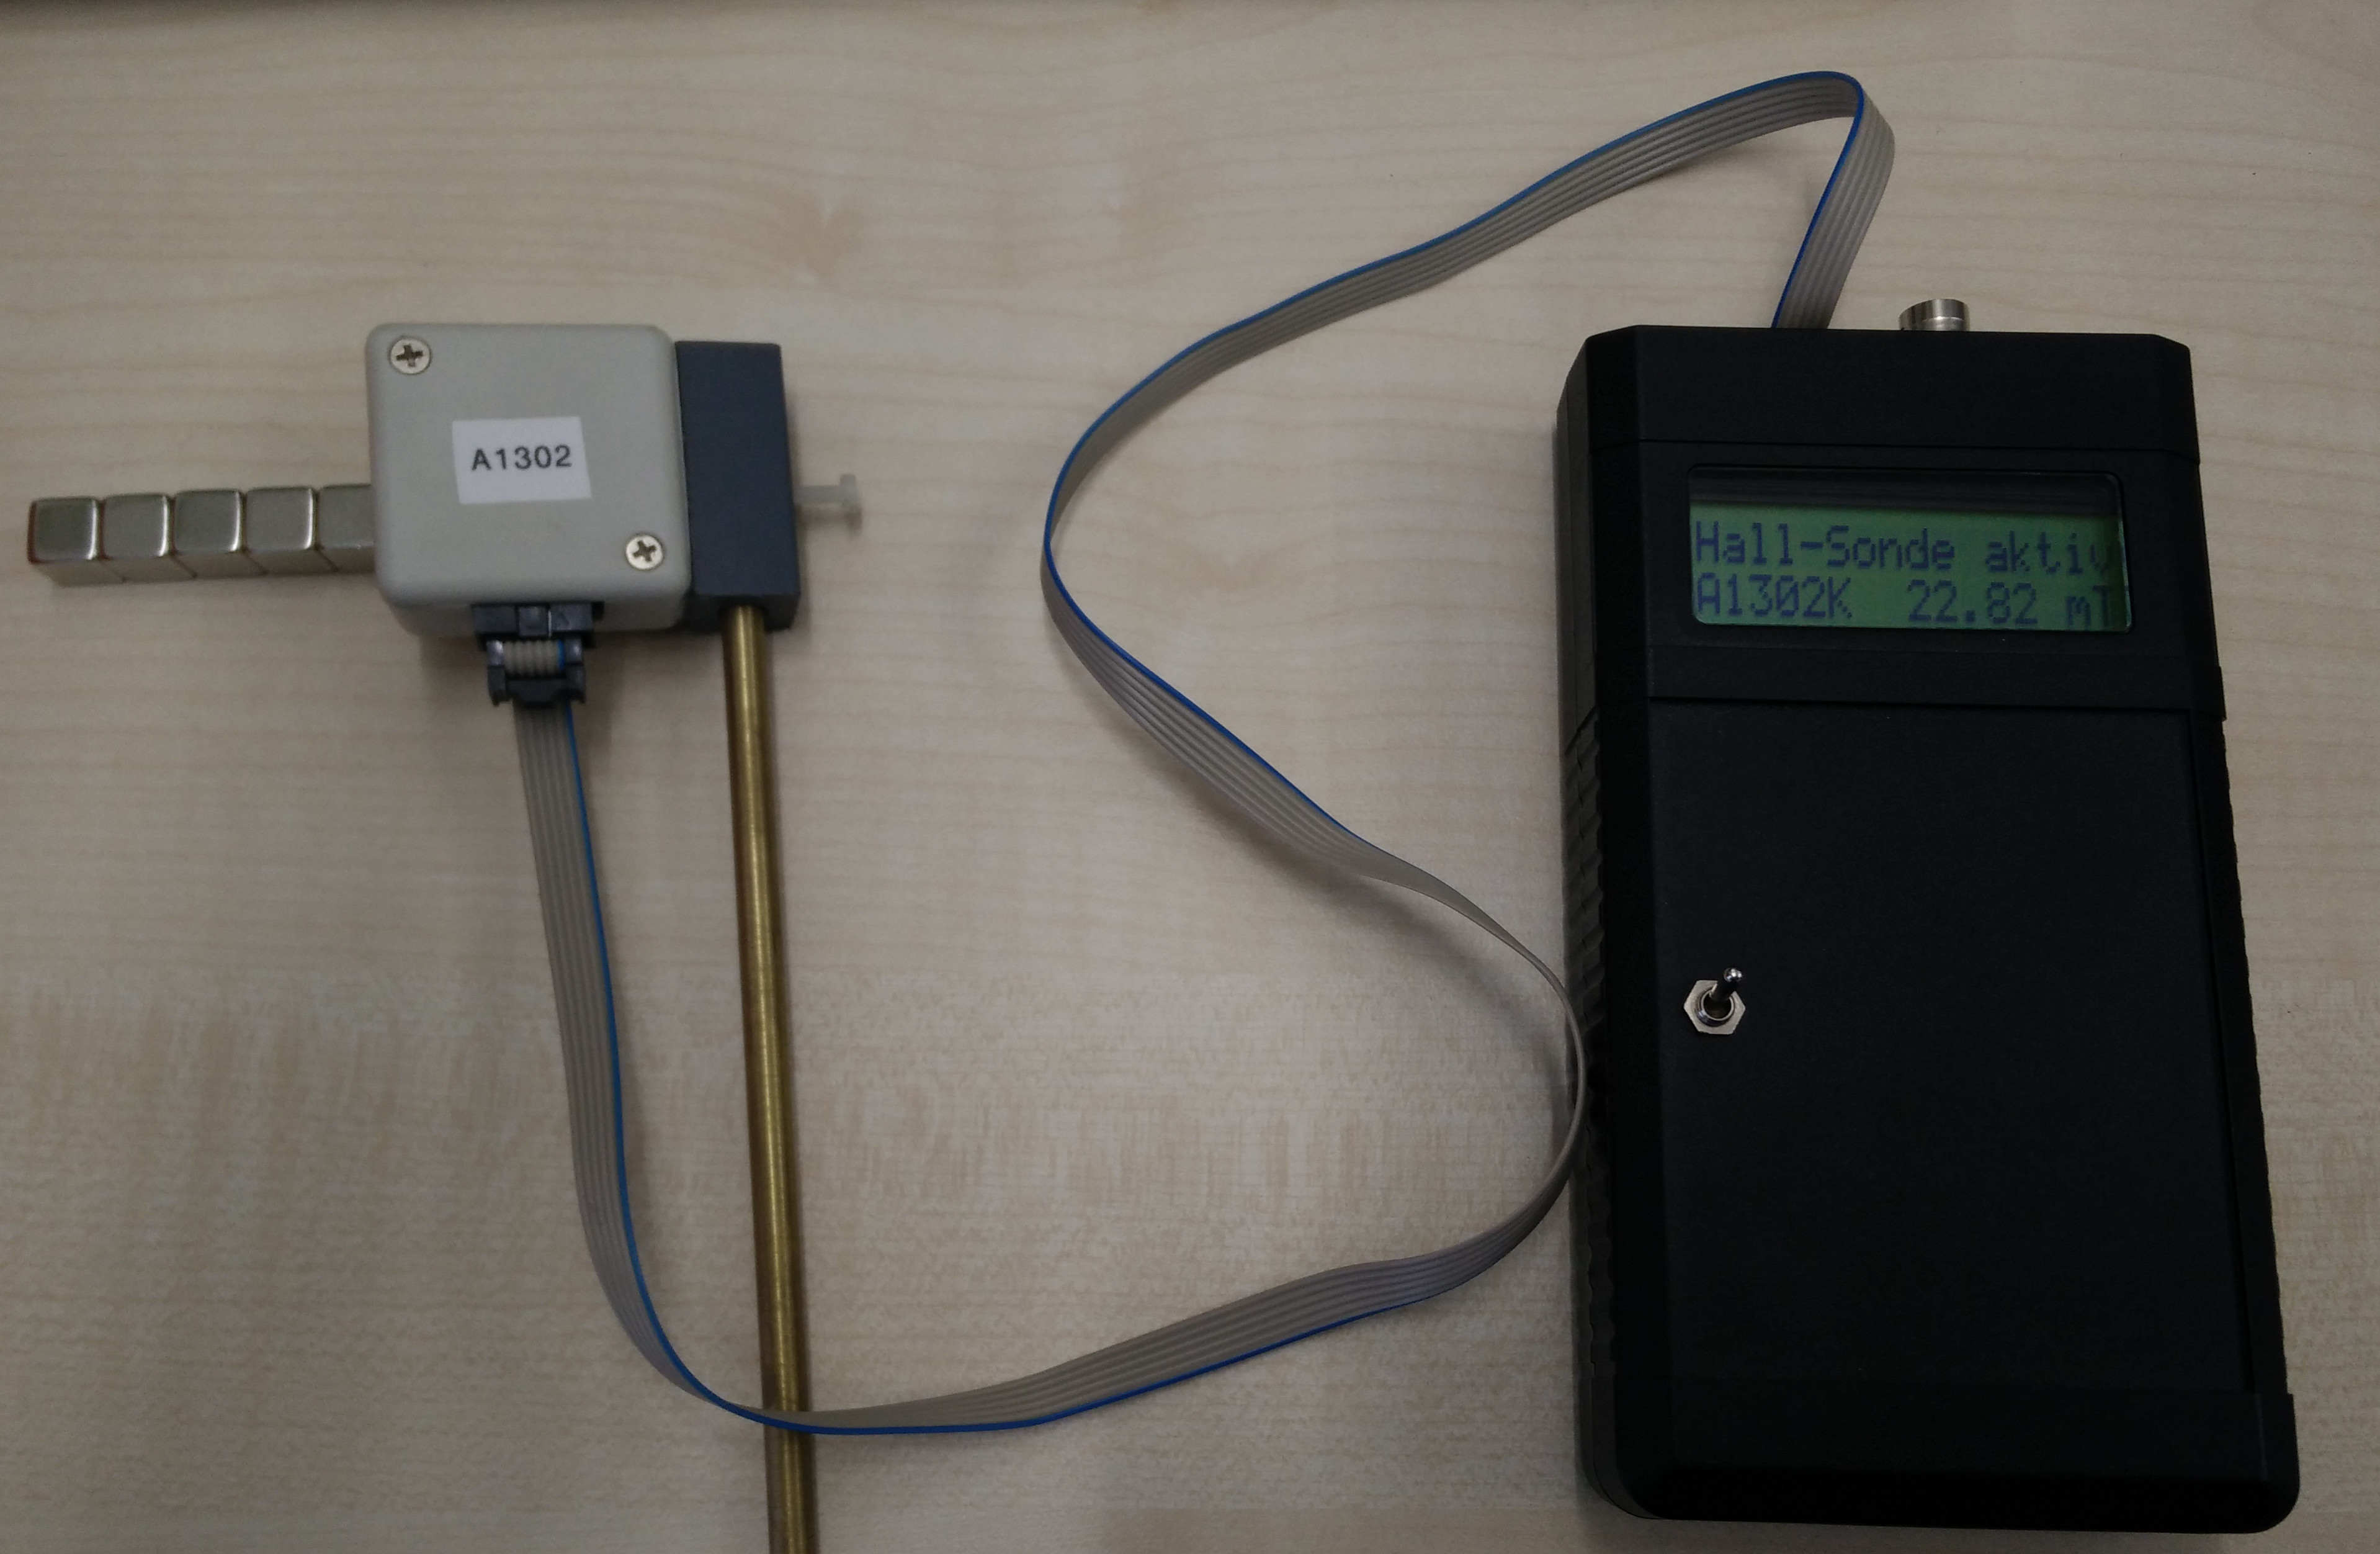
\includegraphics[width=.75\columnwidth]{../pictures/working_with_PM}%
\caption{The handheld hall probe measuring the magnetic flux density of a permanent magnet}%
\label{pic:working_with_PM}%
\end{figure}
A picture of the whole measuring system is presented in \textbf{Figure~\ref{pic:working_with_PM}}.

\subsection{Set of probes}
The magnetic flux density can be measured with different sensitivities. Therefor different hall effect sensors are used. The probes are equipped with ratiometric linear hall effect sensor ICs from \textit{Honeywell} and \textit{Allegro}.
\begin{figure}[ht]%
\centering
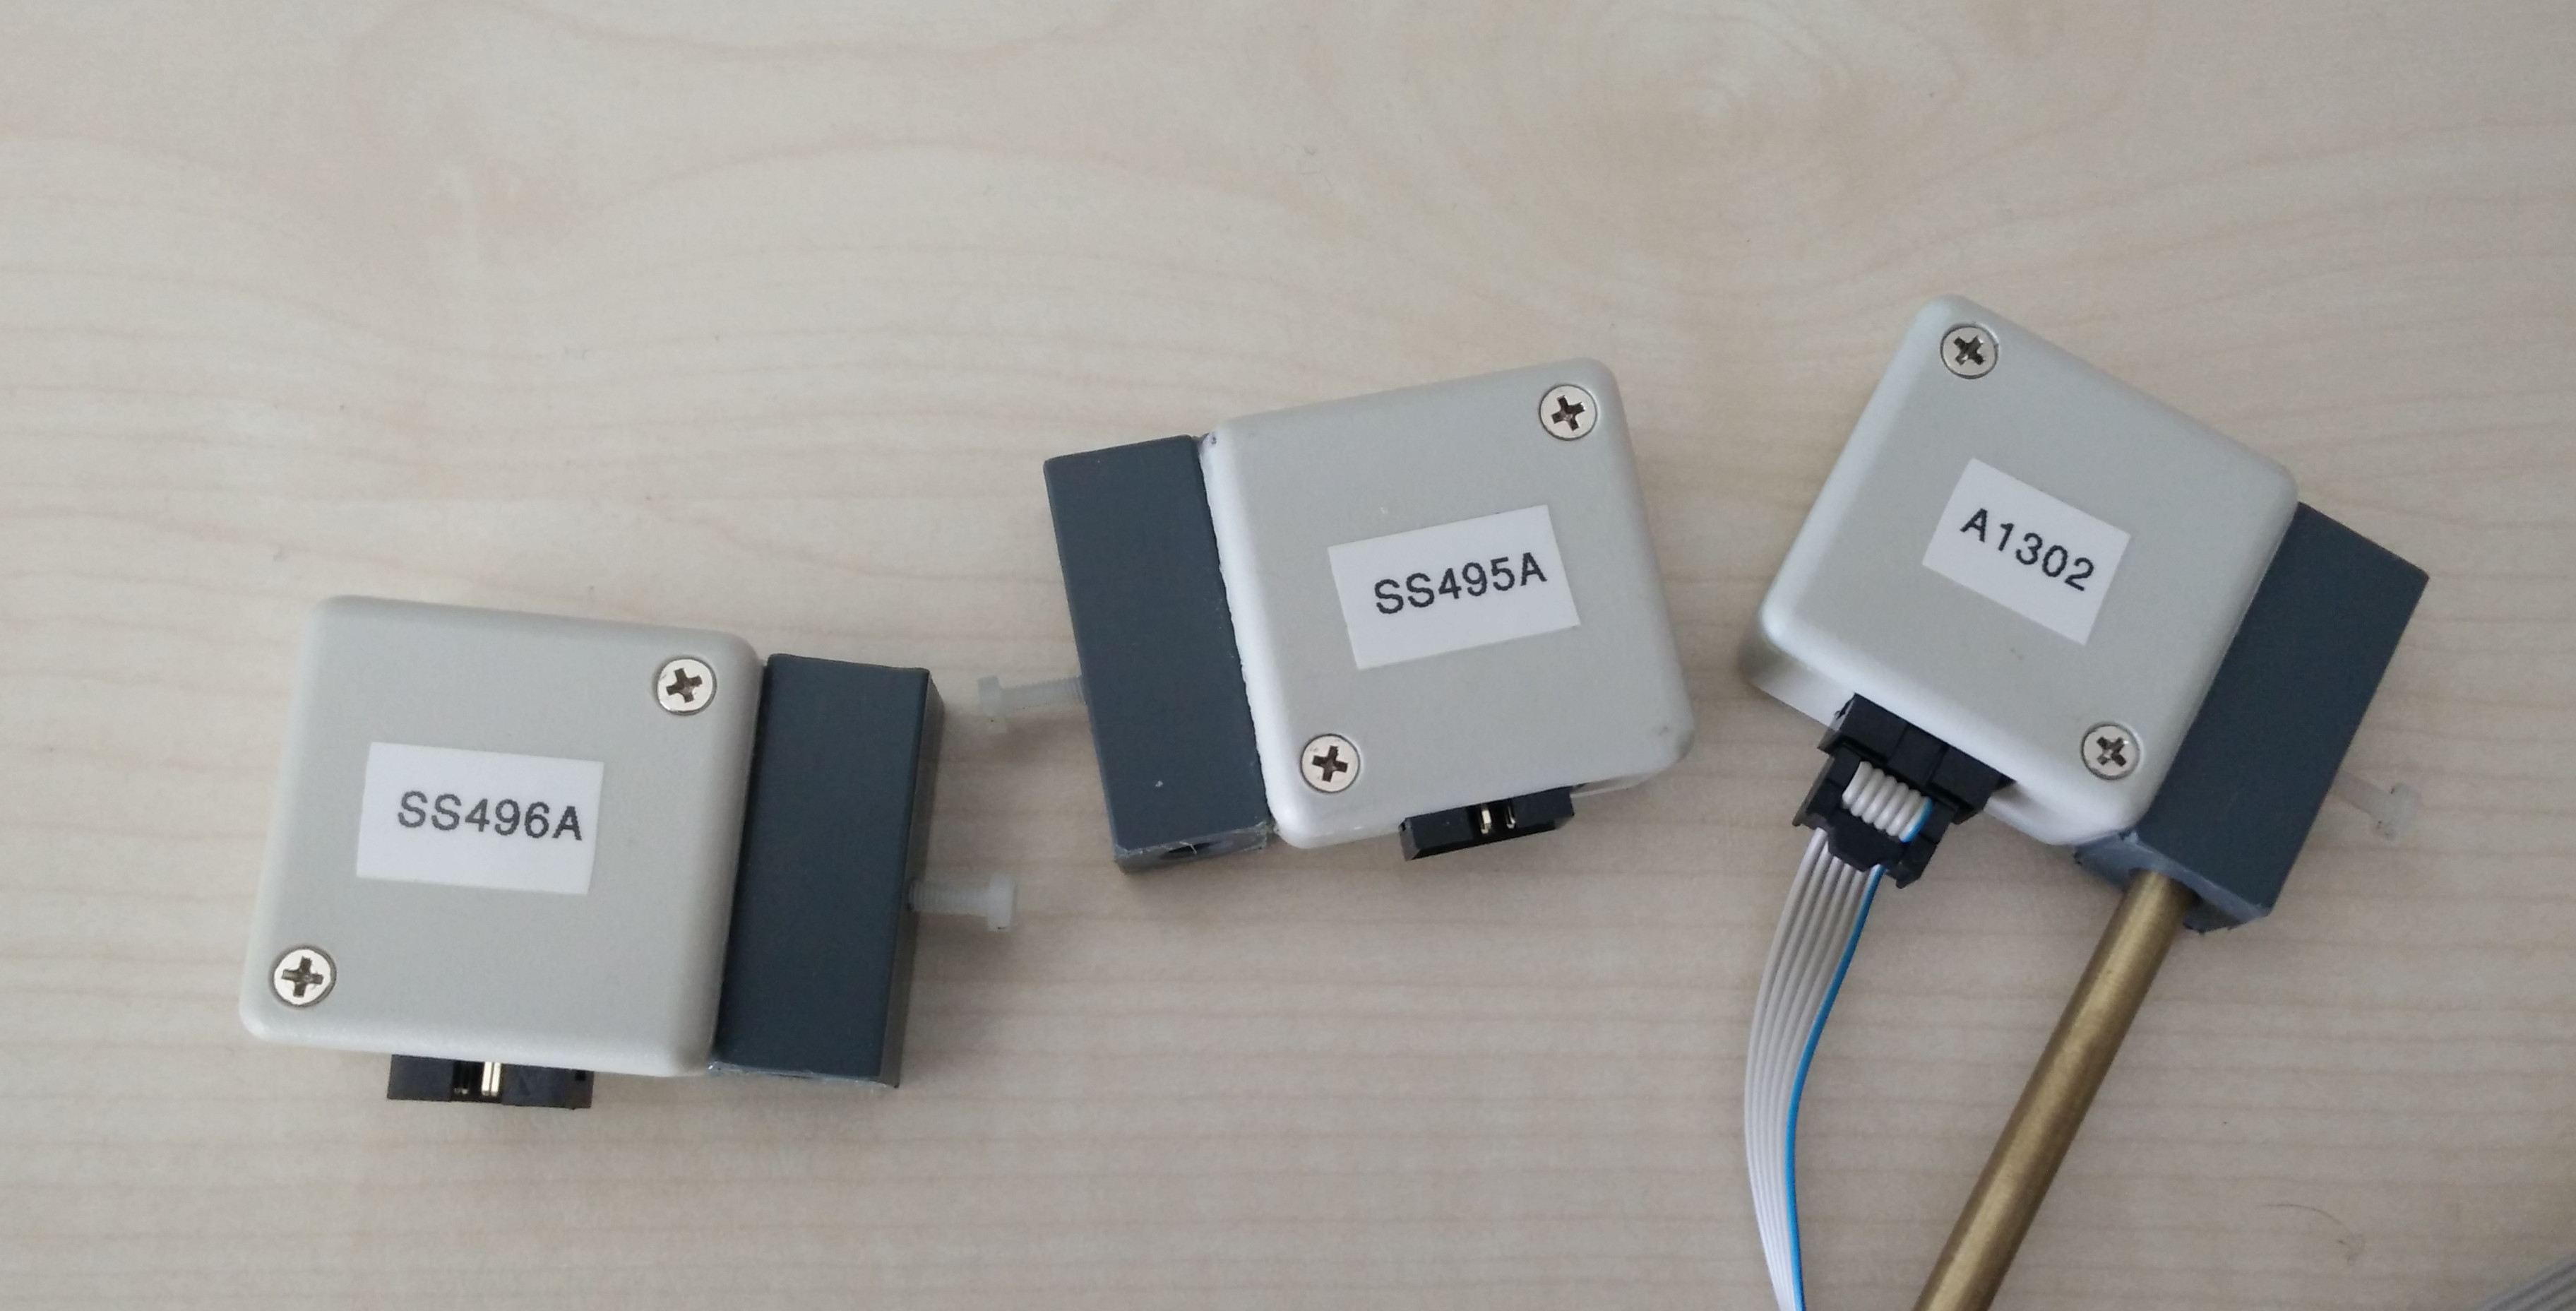
\includegraphics[width=.5\columnwidth]{../pictures/set_of_probes}%
\caption{Three types of sensor chips with different sensitivities can be used}%
\label{pic:set_of_probes}%
\end{figure}
They need a supply voltage of $V_\mathrm{CC} = 5\,\mathrm{V}$ and the output voltage depends linearly from the magnetic flux density. \textbf{Figure~\ref{pic:set_of_probes}} shows the three different sensor in their housings and a rod to hold the device into the measuring area.

\subsection{Connection between measuring probes and handheld device}
\label{chap:connection}
The different probe are connected with the handheld device with a 6-wire-ribbon cable. Two wires are used for the power supply. A third wire connects the voltage output of the hall sensor ICs to the handheld. Two of the remaining three wires are used to identify the different hall sensor ICs and thereby the different sensitivities.

\subsection{The handheld in itself}
The handheld is based on a Arduino Micro and a custom shield. An inside is given by \textbf{Figure~\ref{pic:inside}}.
\begin{figure}[ht]%
\centering
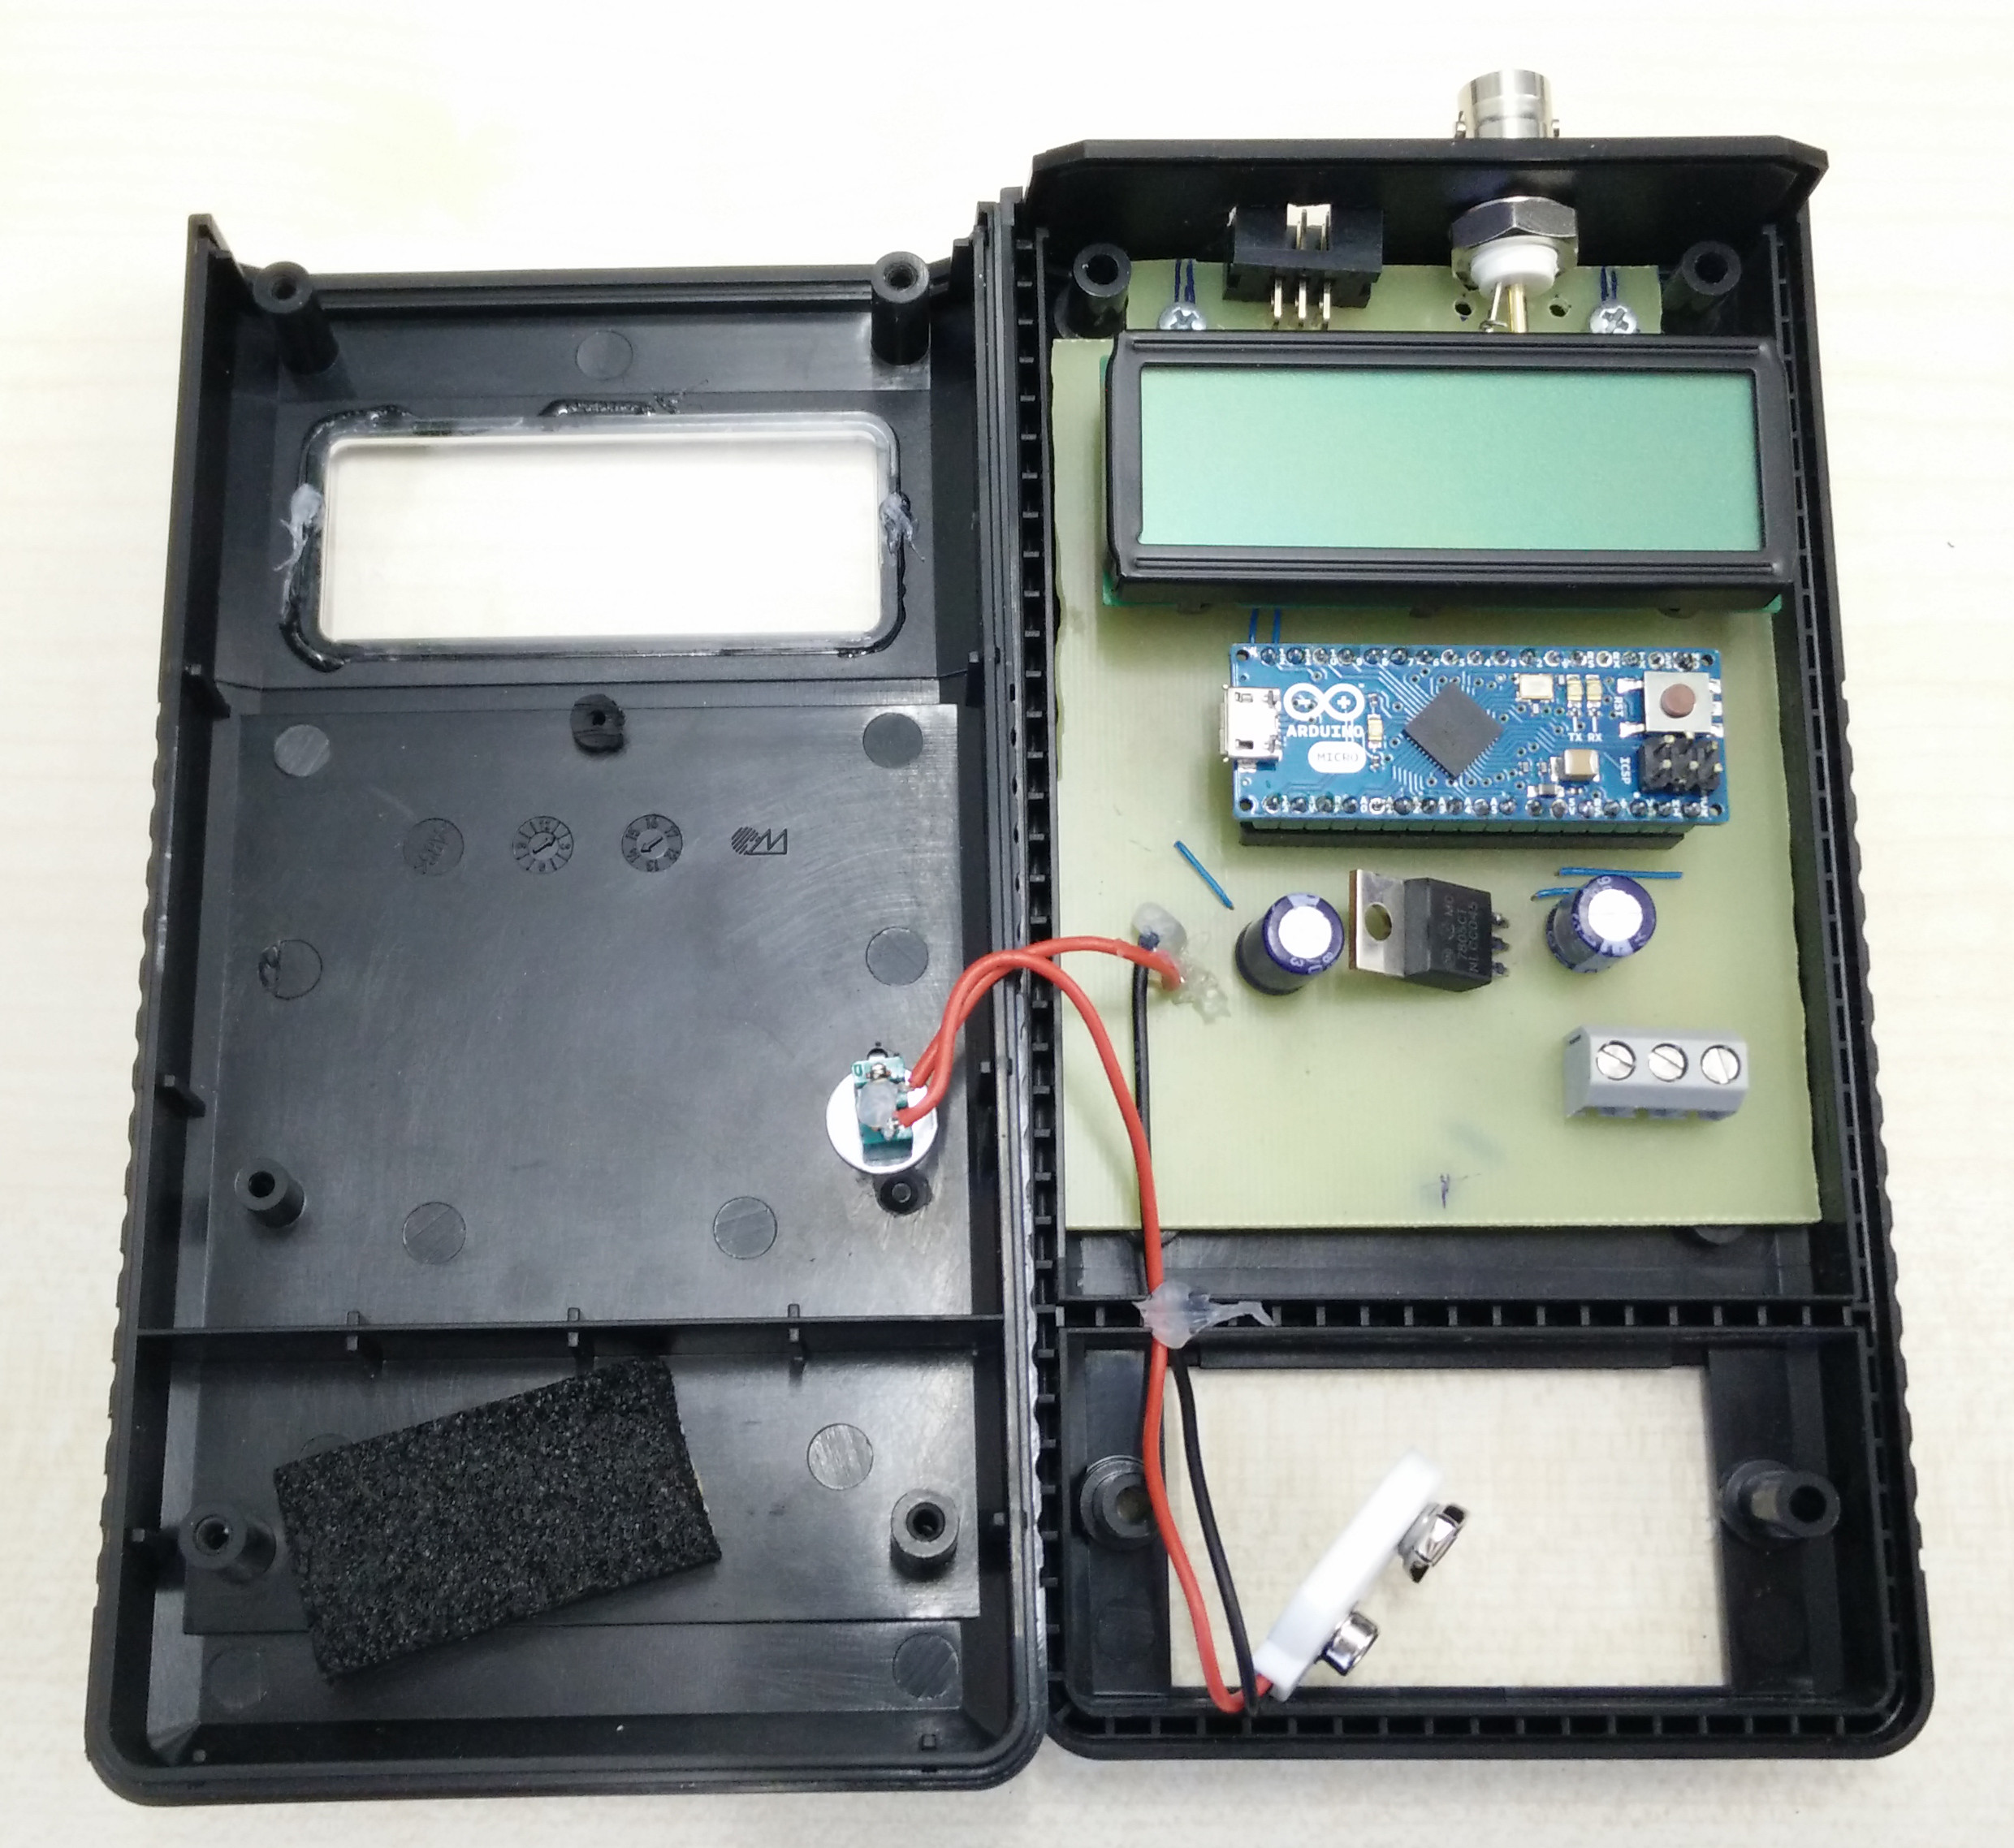
\includegraphics[width=.75\columnwidth]{../pictures/inside}%
\caption{View inside the handheld with the Arduino}%
\label{pic:inside}%
\end{figure}
The device is powered by a nine-volt battery. The voltage for the microcontroller is directly regulated with a 7805 (fixed positive voltage regulator). Thus the Arduino Micro is powered via the port "+5V". The output of the 7805 is also used for the sensor chip, the display and the display background LED, too.
The LCD is connected to the Arduino Micro in 4-bit mode and without the "rw contol" to minimise the wiring effort.
As already mentioned in \textbf{Chapter~\ref{chap:connection}} the Arduino Micro can check automatically which sensor is linked. Therefor two digital ports are used to detect whether the corresponding channel is pulled to ground or $5\,\mathrm{V}$. The measured signal is connected to the analog port "A0".
The schematic of the developed shield can be found in \textbf{Appendix~\ref{app:schematic}}. The PCB layout was designed with EAGLE. It is shown in \textbf{Appendix~\ref{app:board}}.

\section{Software}

The Arduino Micro is flashed by the USB port with the Arduino IDE and Arduino code. The complete code is attached to \textbf{Appendix~\ref{app:code}}.
The LCD is controled by the Arduino Micro using the \texttt{LiquidCrystal Library}. For timing purposes the \texttt{TimerNull Library} is used. It provides the functionality of the timer interrupts of the ATmega~32U4.
To access the measured data the variables are initialised as \texttt{volatile}.

\subsection{The \texttt{setup()} function}
Within the \texttt{setup()} function the LCD will be started and static data will be written.

The measurement should be performed with an averaging. Every single point of measurement shall be taken every $50\,\upmu\mathrm{s}$. For this reason the timer interrupt will be set to this time and be attached as interrupt.

\subsection{The \texttt{loop()} function}
Nothing will be perfomed. The Arduino Micro is just waiting for instructions from the timer interrupt.

\subsection{The \texttt{readHall()} function and the sub-functions}
Every times the timer interrupts the magnetic flux density will be measured and stored in a collection of all current measuring values. The number of all measuring values is increased by one. When 5000 measurements are performed the average will be calculated and shown on the display. To be able to measure also alternating fields the rms-value will be used as averaging method:
$$B_\mathrm{rms} = \sqrt{\frac{\sum_{i=1}^{n=5000}{\left(\frac{\frac{U_{\mathrm{in},i}}{1023}\cdot 5000-U_\mathrm{ref}}{k_\mathrm{divider}}\right)^2}}{5000}}$$
\begin{itemize}
	\item[$U_{\mathrm{in},i}$:] value returned by \texttt{analogRead()}
	\item[$U_\mathrm{ref}$:] reference voltage which is returned by sensor at $B=0\,\mathrm{T}$
	\item[$k_\mathrm{divider}$:] divider to convert measured voltage into a flux density, unit: $\mathrm{\frac{mV}{mT}}$
\end{itemize}
The values $U_\mathrm{ref}$ and $k_\mathrm{divider}$ depend on the type of hall sensor IC and will be set by the function \texttt{setSensorTyp()}. This functions evaluates the digital status (\texttt{HIGH} or \texttt{LOW}) on the inputs "A2"' and "A3" and sets the sensor specific values to the volatile variables. If no sensor is identified an error is returned to the customer: \texttt{Sensor?}.

Finally the measured magnetic flux density will be shown on the display.




\newpage
\renewcommand*{\thesubsection}{\Roman{subsection}}
\section{Appendix}

\subsection{The Arduino code}
\label{app:code}
\lstset{language=C++,%
	numbers=left,%
	basicstyle=\small,%
	numberstyle=\tiny,%
	breaklines=true}
\lstinputlisting[frame=single]{../Code/Hallsonde/Hallsonde.ino}


\subsection{Schematic of the shield}
\label{app:schematic}
\begin{figure}[h]%
\centering
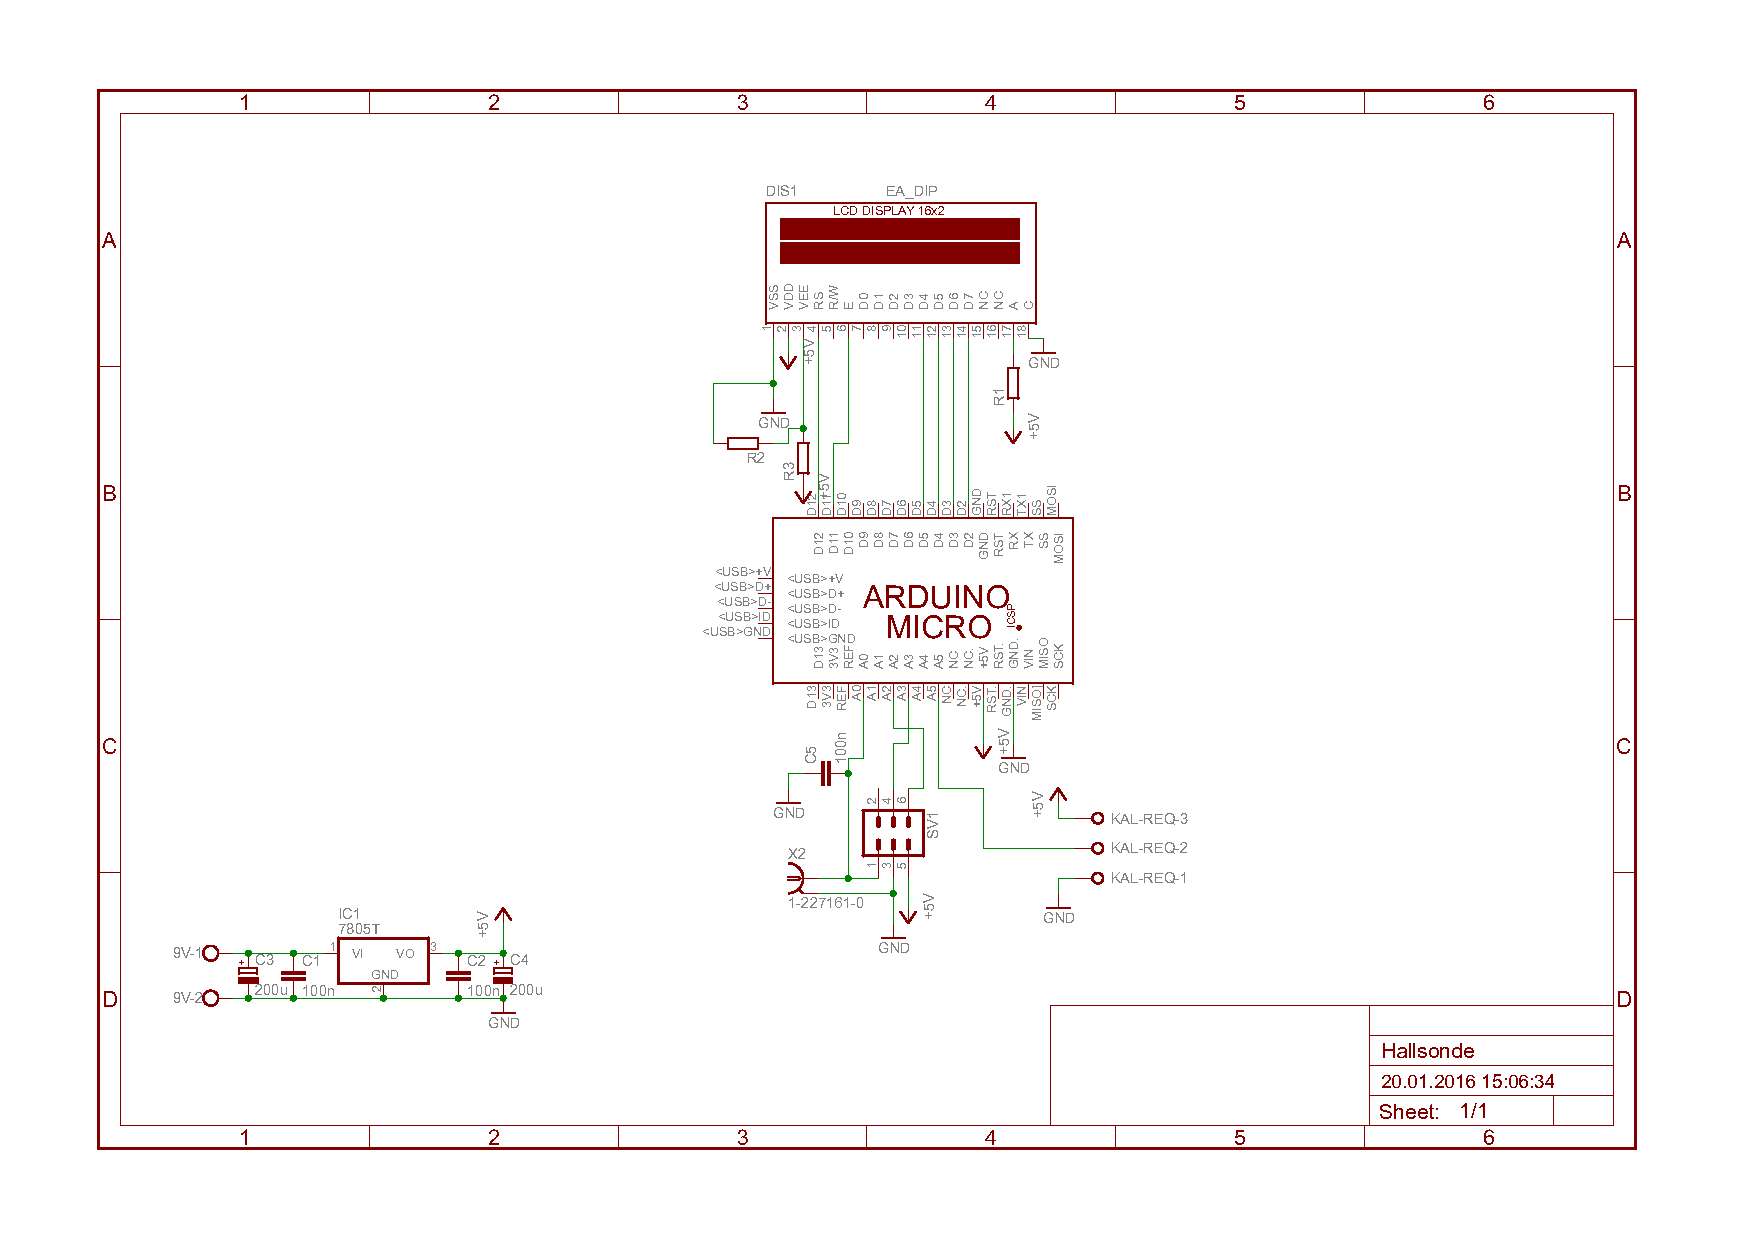
\includegraphics[width=.75\textheight,angle=90]{../Layout/Hallsonde_Schematic}%
\end{figure}

\newpage
\subsection{Layout of the PCB}
\label{app:board}
\begin{figure}[h]%
\centering
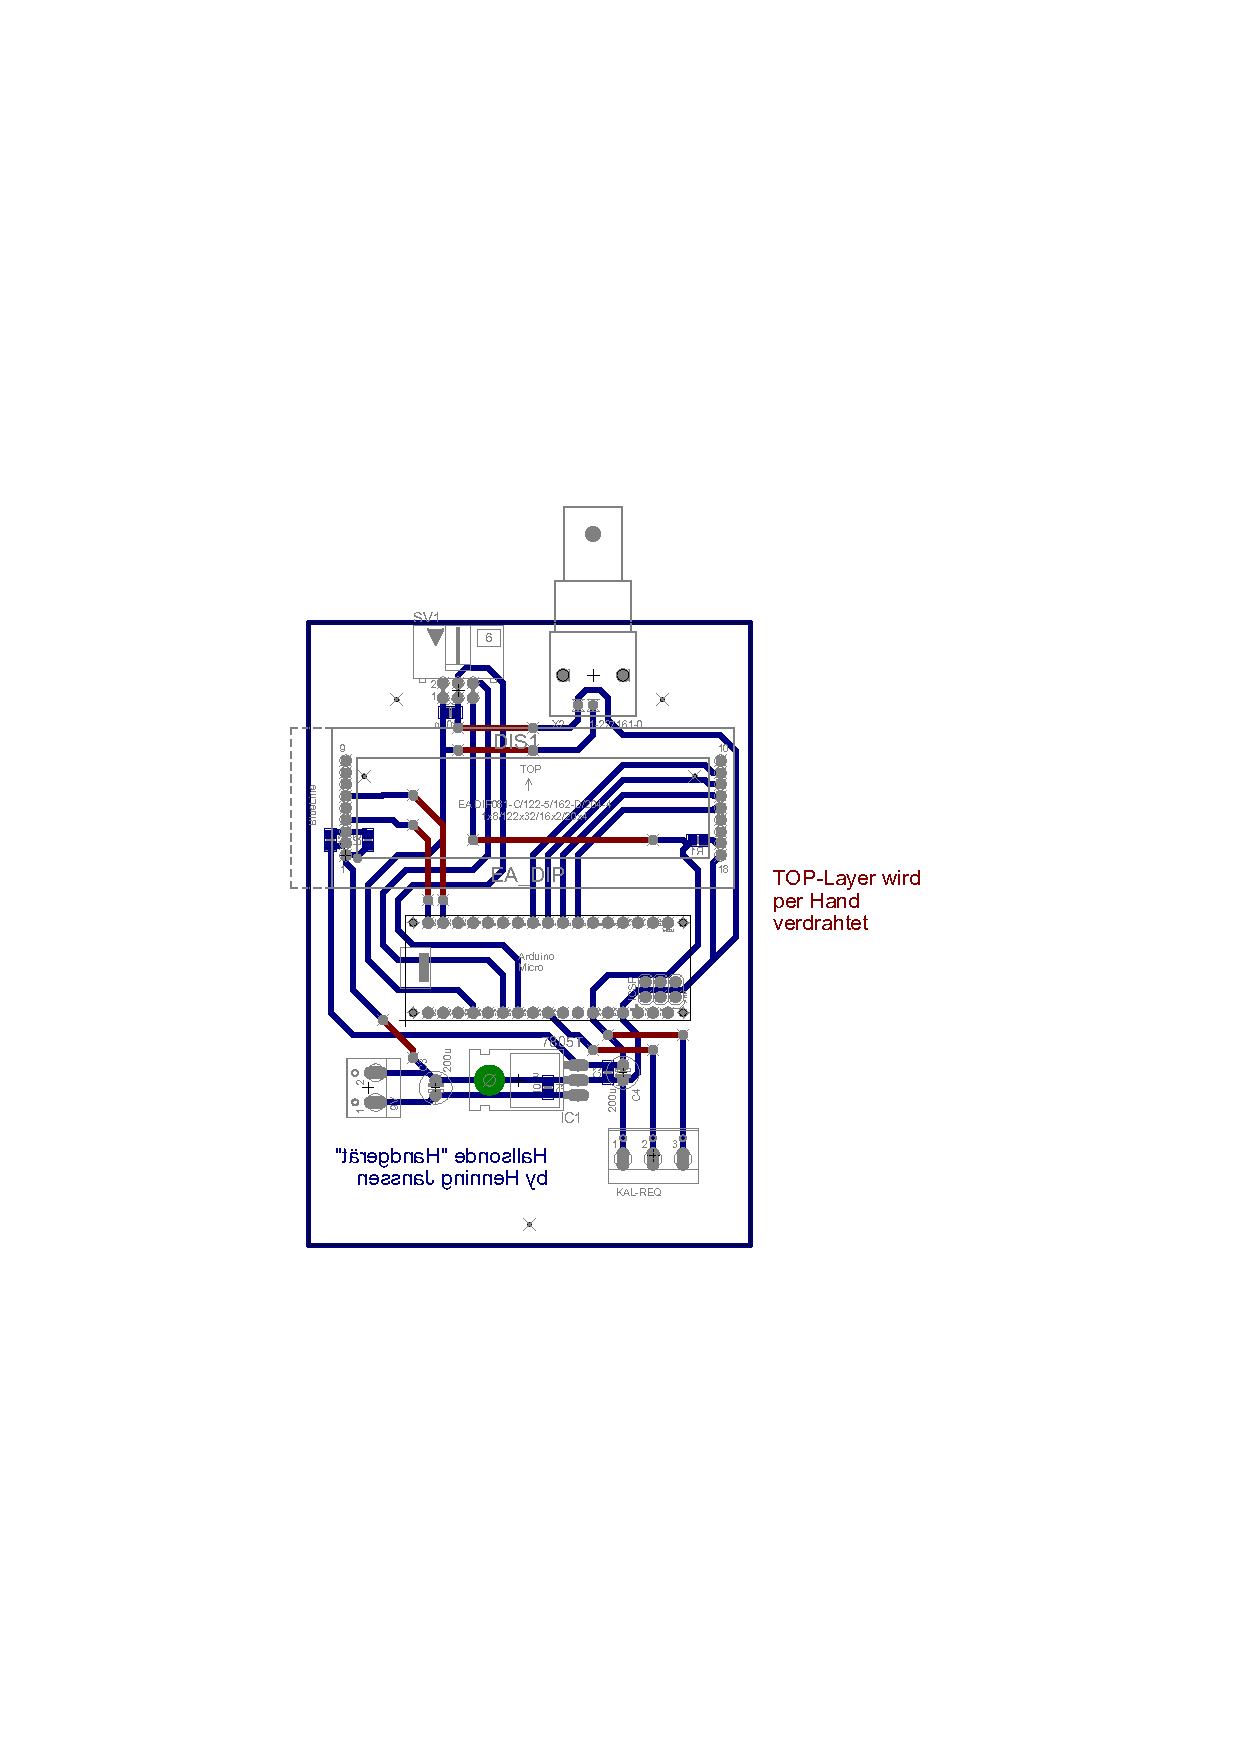
\includegraphics[angle=90]{../Layout/Hallsonde_board}%
\end{figure}


\end{document}